\documentclass{hitec}
\author{FOSSEE, IIT Bombay}
\title{Flashing Modelica Code to and Arduino using MDD}

\usepackage{forest}
\usepackage{graphicx}
\usepackage[T1]{fontenc}
\usepackage[utf8]{inputenc}
\usepackage{lmodern,hyperref,graphicx,tcolorbox,listings,fancyhdr,longtable,caption,color,dblfnote}
\usepackage[titletoc]{appendix}
\usepackage[english]{babel}

\begin{document}
\maketitle
\section{Introduction}
This document has been written with the intent of familiarising a user with the aspects of the Modelica Device Drivers (MDD) package that allow one to flash OpenModelica code directly to an Arduino.  

This article will briefly cover the usage of the Embedded Targets subpackage within Modelica Device Drivers package and will then detail a specific example.
\
\section{Usage}
MDD consists of a variety of ways of communicating with external devices, but one of its most powerful utilities is the ability to create flashable C files for AVR and STM microcontrollers. This allows users with little experience in AVR C to code instructions to the microcontroller. While the steps for this haven't entirely been integrated within OpenModelica itself, they are fairly straightforward and with the usage of an example, we will explain them below.
\\
Before we begin, we will need the following tools. This doc assumes that the user is using a linux based system. If the user has Ubuntu installed, they should run the following commands to install the relevant tools for the task.

\begin{itemize}
\item sudo apt-get install gcc-avr
\item sudo apt-get install avr-libc
\item sudo apt-get install avrdude
\end{itemize}

The experiment being done is that of turning an LED on with two different colours within a 10 second interval. The shield being used for this looks as given below:
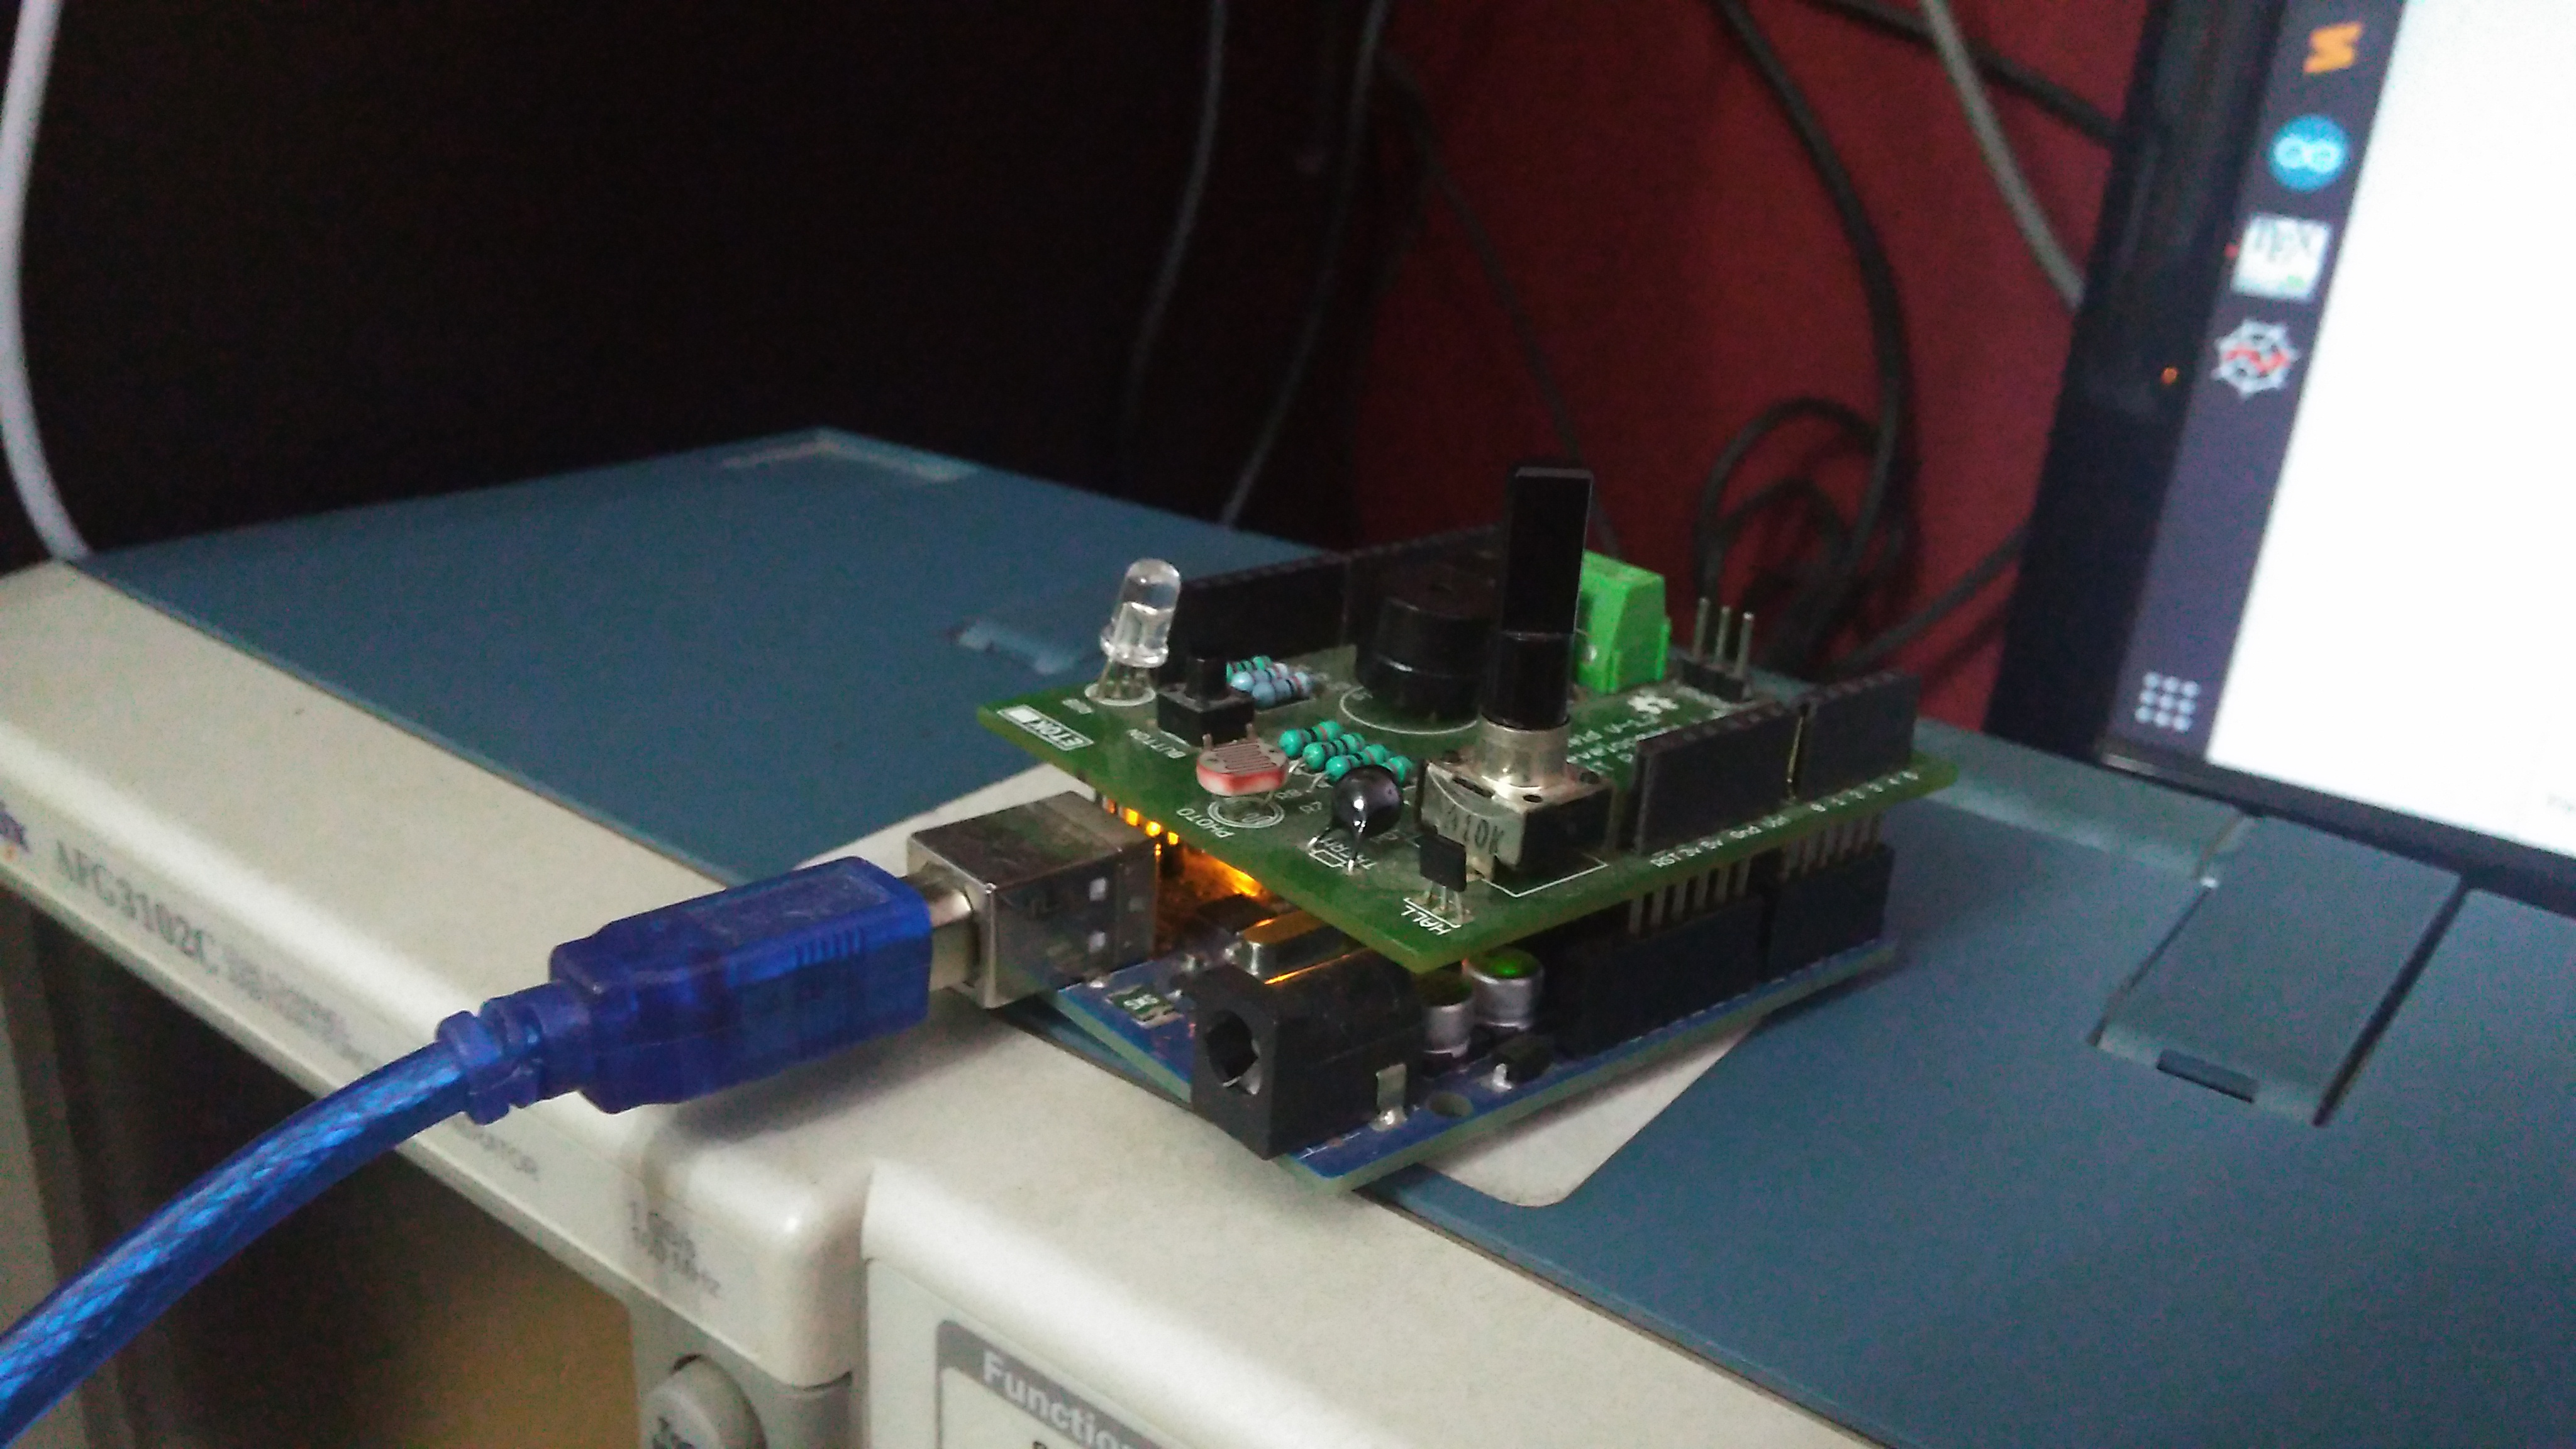
\includegraphics[scale=0.1]{Image_Of_Shield.jpg}

The model that will be uploaded looks as given below:
\begin{center}
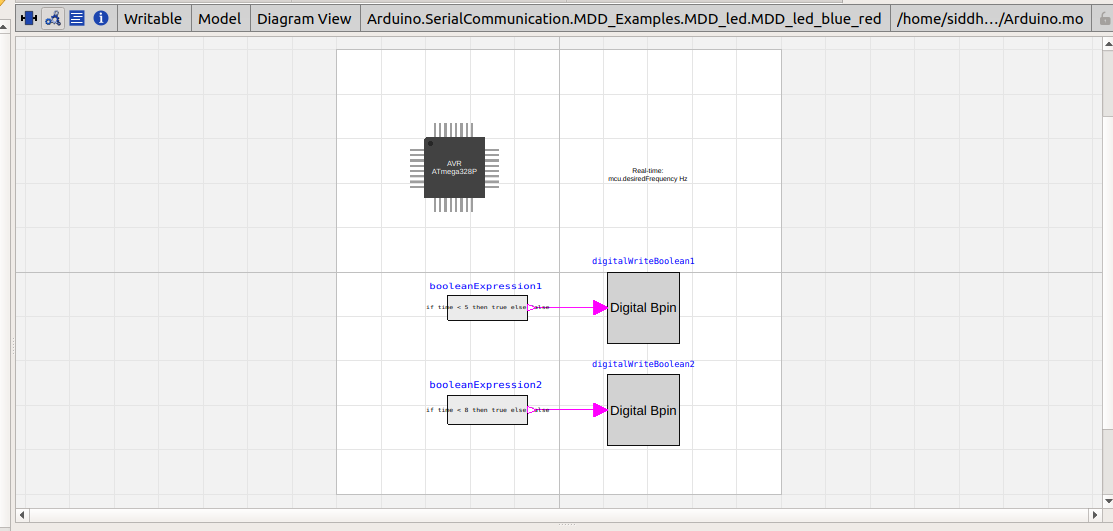
\includegraphics[scale=0.25]{Model.png}
\end{center}

The model consists of an embedded block with pre-defined parameters for the ATmega328P microcontroller. It can be modified to suit any ATMel controller, provided the user knows its characteristics. This block is unconnected to any other in the model.
\\
\\
Now we look at the blocks that specify the task to be done. The boolean expression blocks have fairly simple utility here. They are just modifying their state based on the time. The Digital Write Boolean pins communicate the state of the Boolean expression blocks to the pins specified, which are in turn connected to the shield and allow for the LED light colour to change.
\\
\\
Next, we create a .mos file for the problem at hand. As we mentioned before, we can't directly flash the model to the arduino, so we will be doing it via the terminal. The first step involves creating a .mos file that will load the relevant files in memory and then translate the model into a C file. A generic .mos script is shown below
\begin{lstlisting}
loadModel(Modelica);
getErrorString();

loadFile("/home/[path to Modelica_DeviceDrivers]/Modelica_DeviceDrivers/package.mo");
getErrorString();

loadFile("/home/[path to the package containing the example]/package.mo");
getErrorString();

translateModel(package.subpackage.example, fileNamePrefix="[file_prefix_of_choice]");
getErrorString();
\end{lstlisting}

After the file is created, execute the following steps. Since the example we are using here is called led\_ blue \_red, that is the name we are going with in the steps.
\\
\begin{itemize}
\item  omc --simCodeTarget=ExperimentalEmbeddedC runMDD\_ led\_ blue\_ red.mos
\item avr-gcc -Os -std=c11 -ffunction-sections -fdata-sections -mmcu=atmega328p -DF\_ CPU=16000000UL -Wl,--gc-sections led\_ blue\_ red\_ main.c -o led\_ blue\_ red -I /path\_ to\_ MDD/Modelica\_ DeviceDrivers/Resources/Include -I /usr/include/omc/c
\item  avr-objcopy -O ihex -R .eeprom led\_ blue\_ red led\_ blue\_ red.hex
\item avrdude -F -V -c arduino -p ATMEGA328P -P /dev/ttyACM0 -b 115200 -U flash:w:led\_ blue\_ red.hex

\end{itemize}

On doing so, the LED on the shield will light up, first with a bluish colour and then with a red colour as shown in the images below. 


\begin{center}
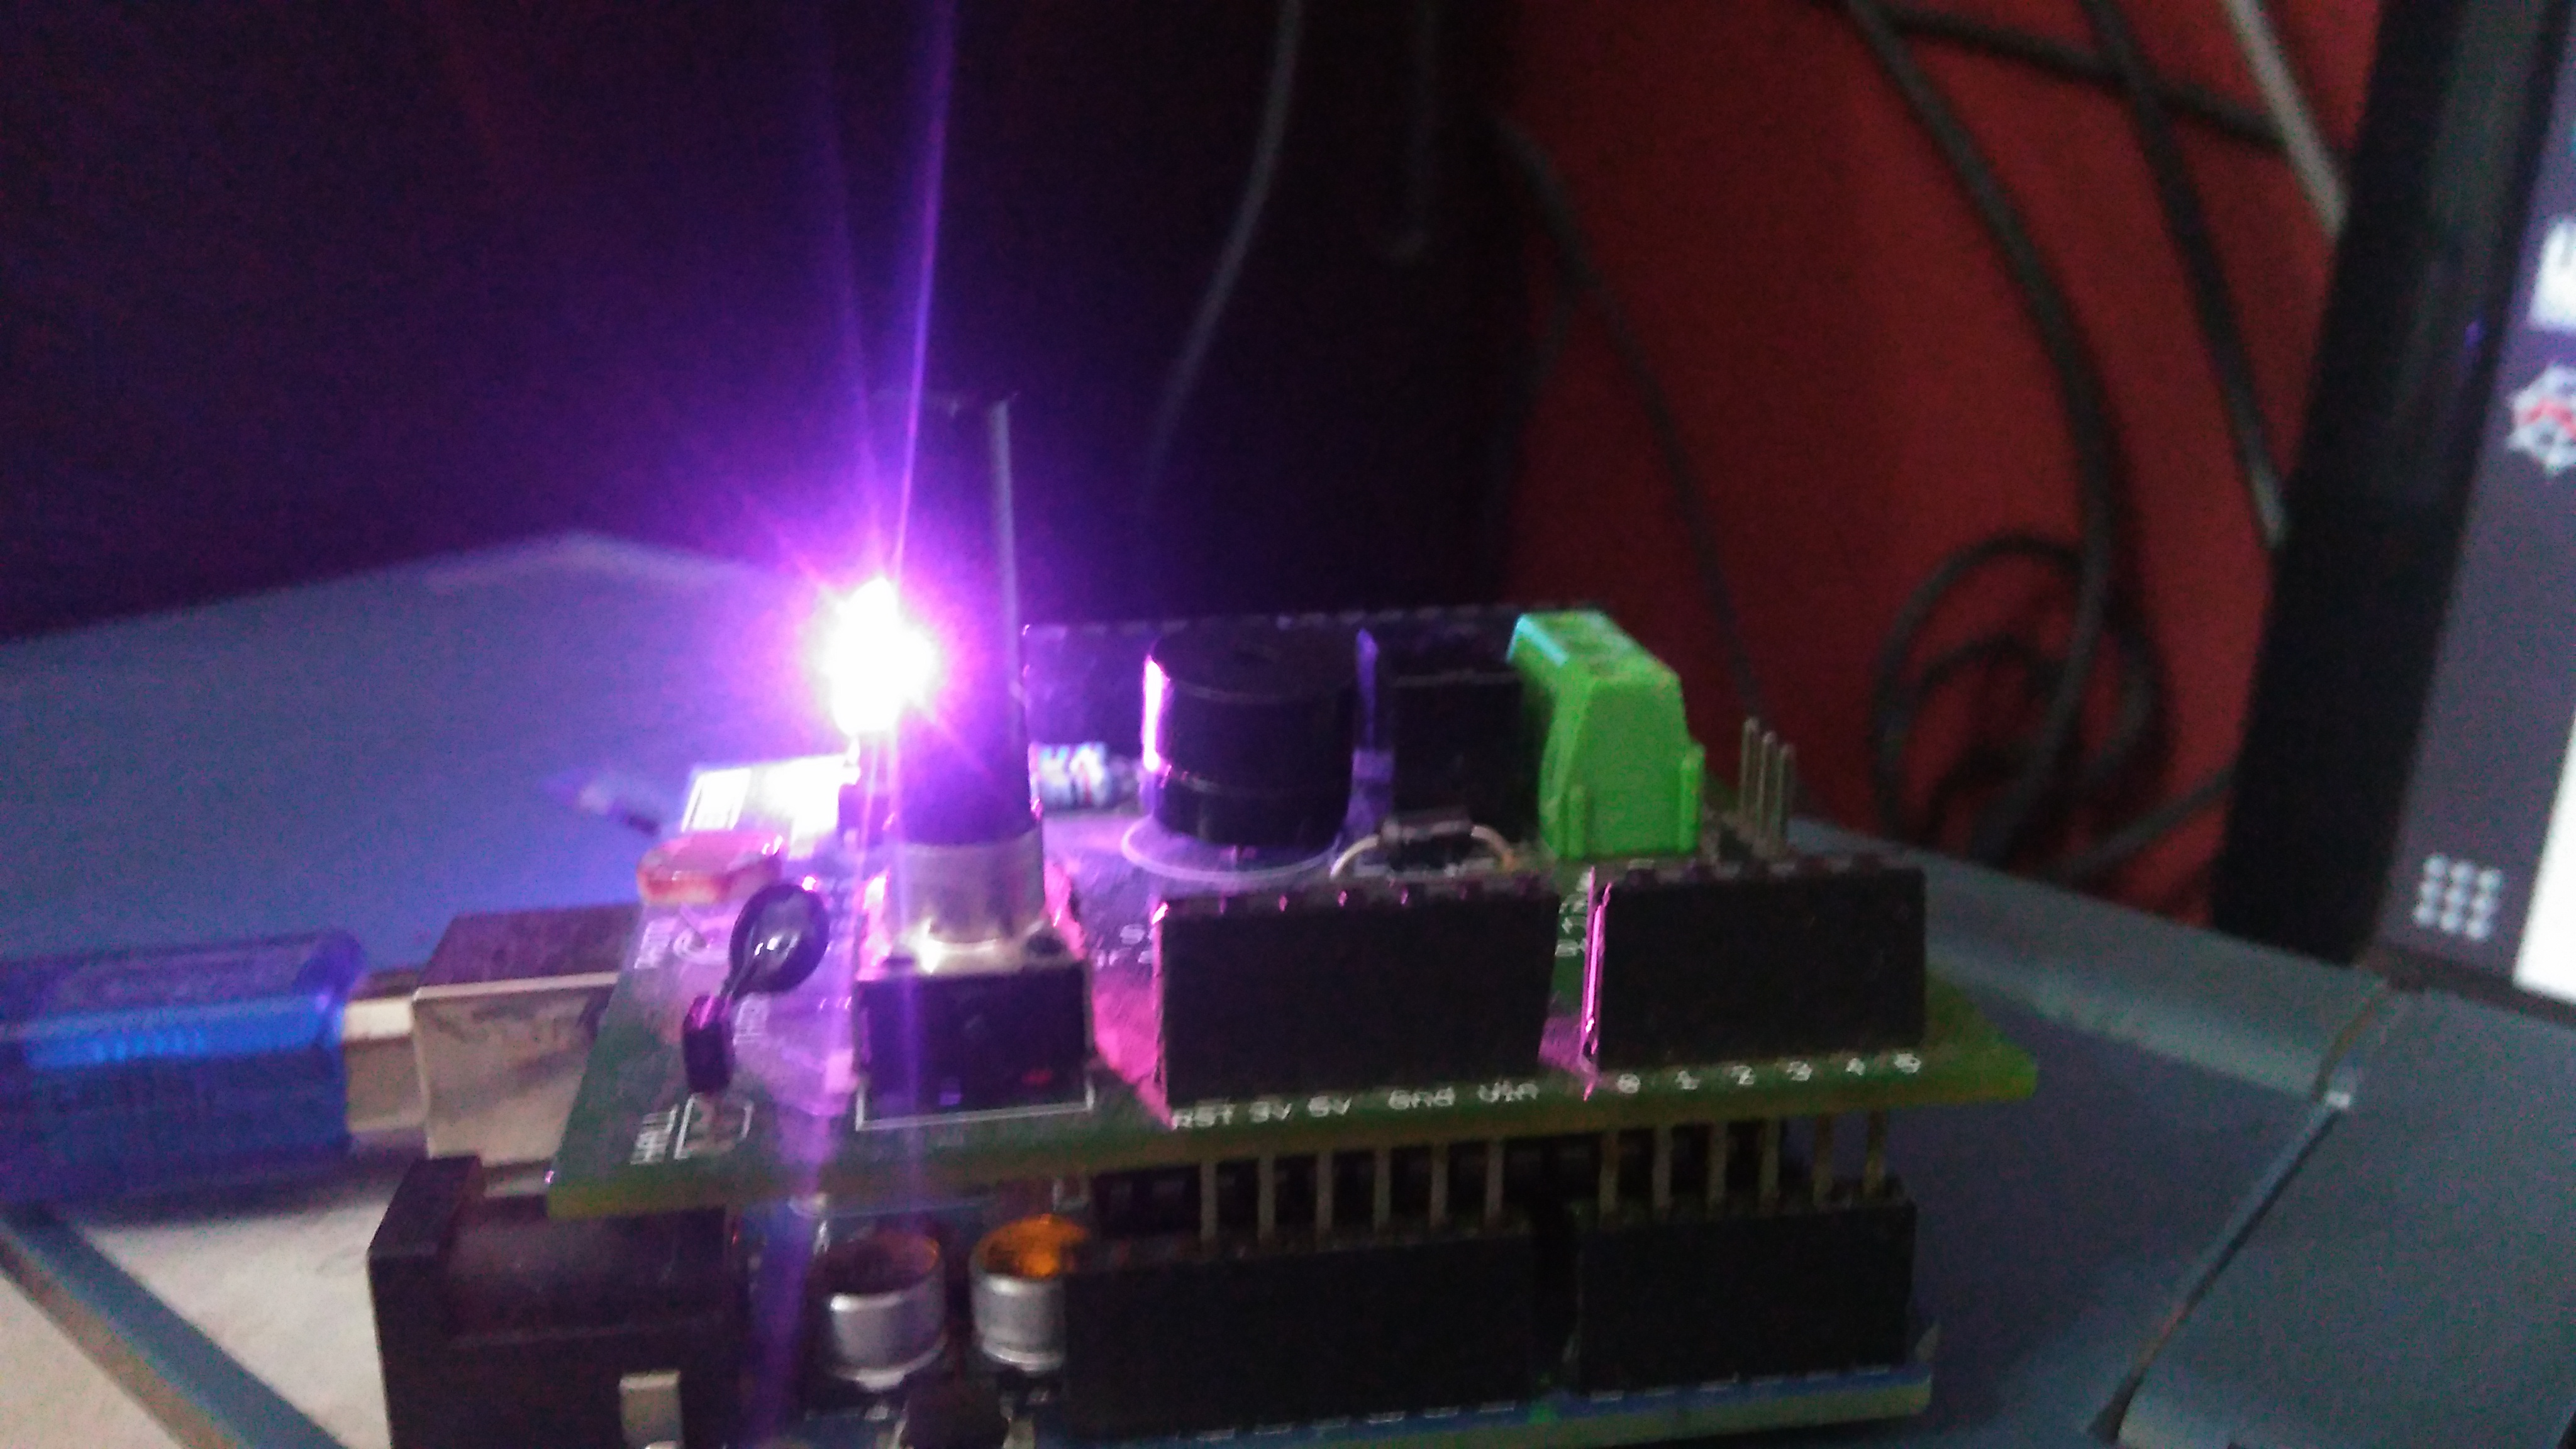
\includegraphics[scale=0.1]{IMG_20180427_131831.jpg}
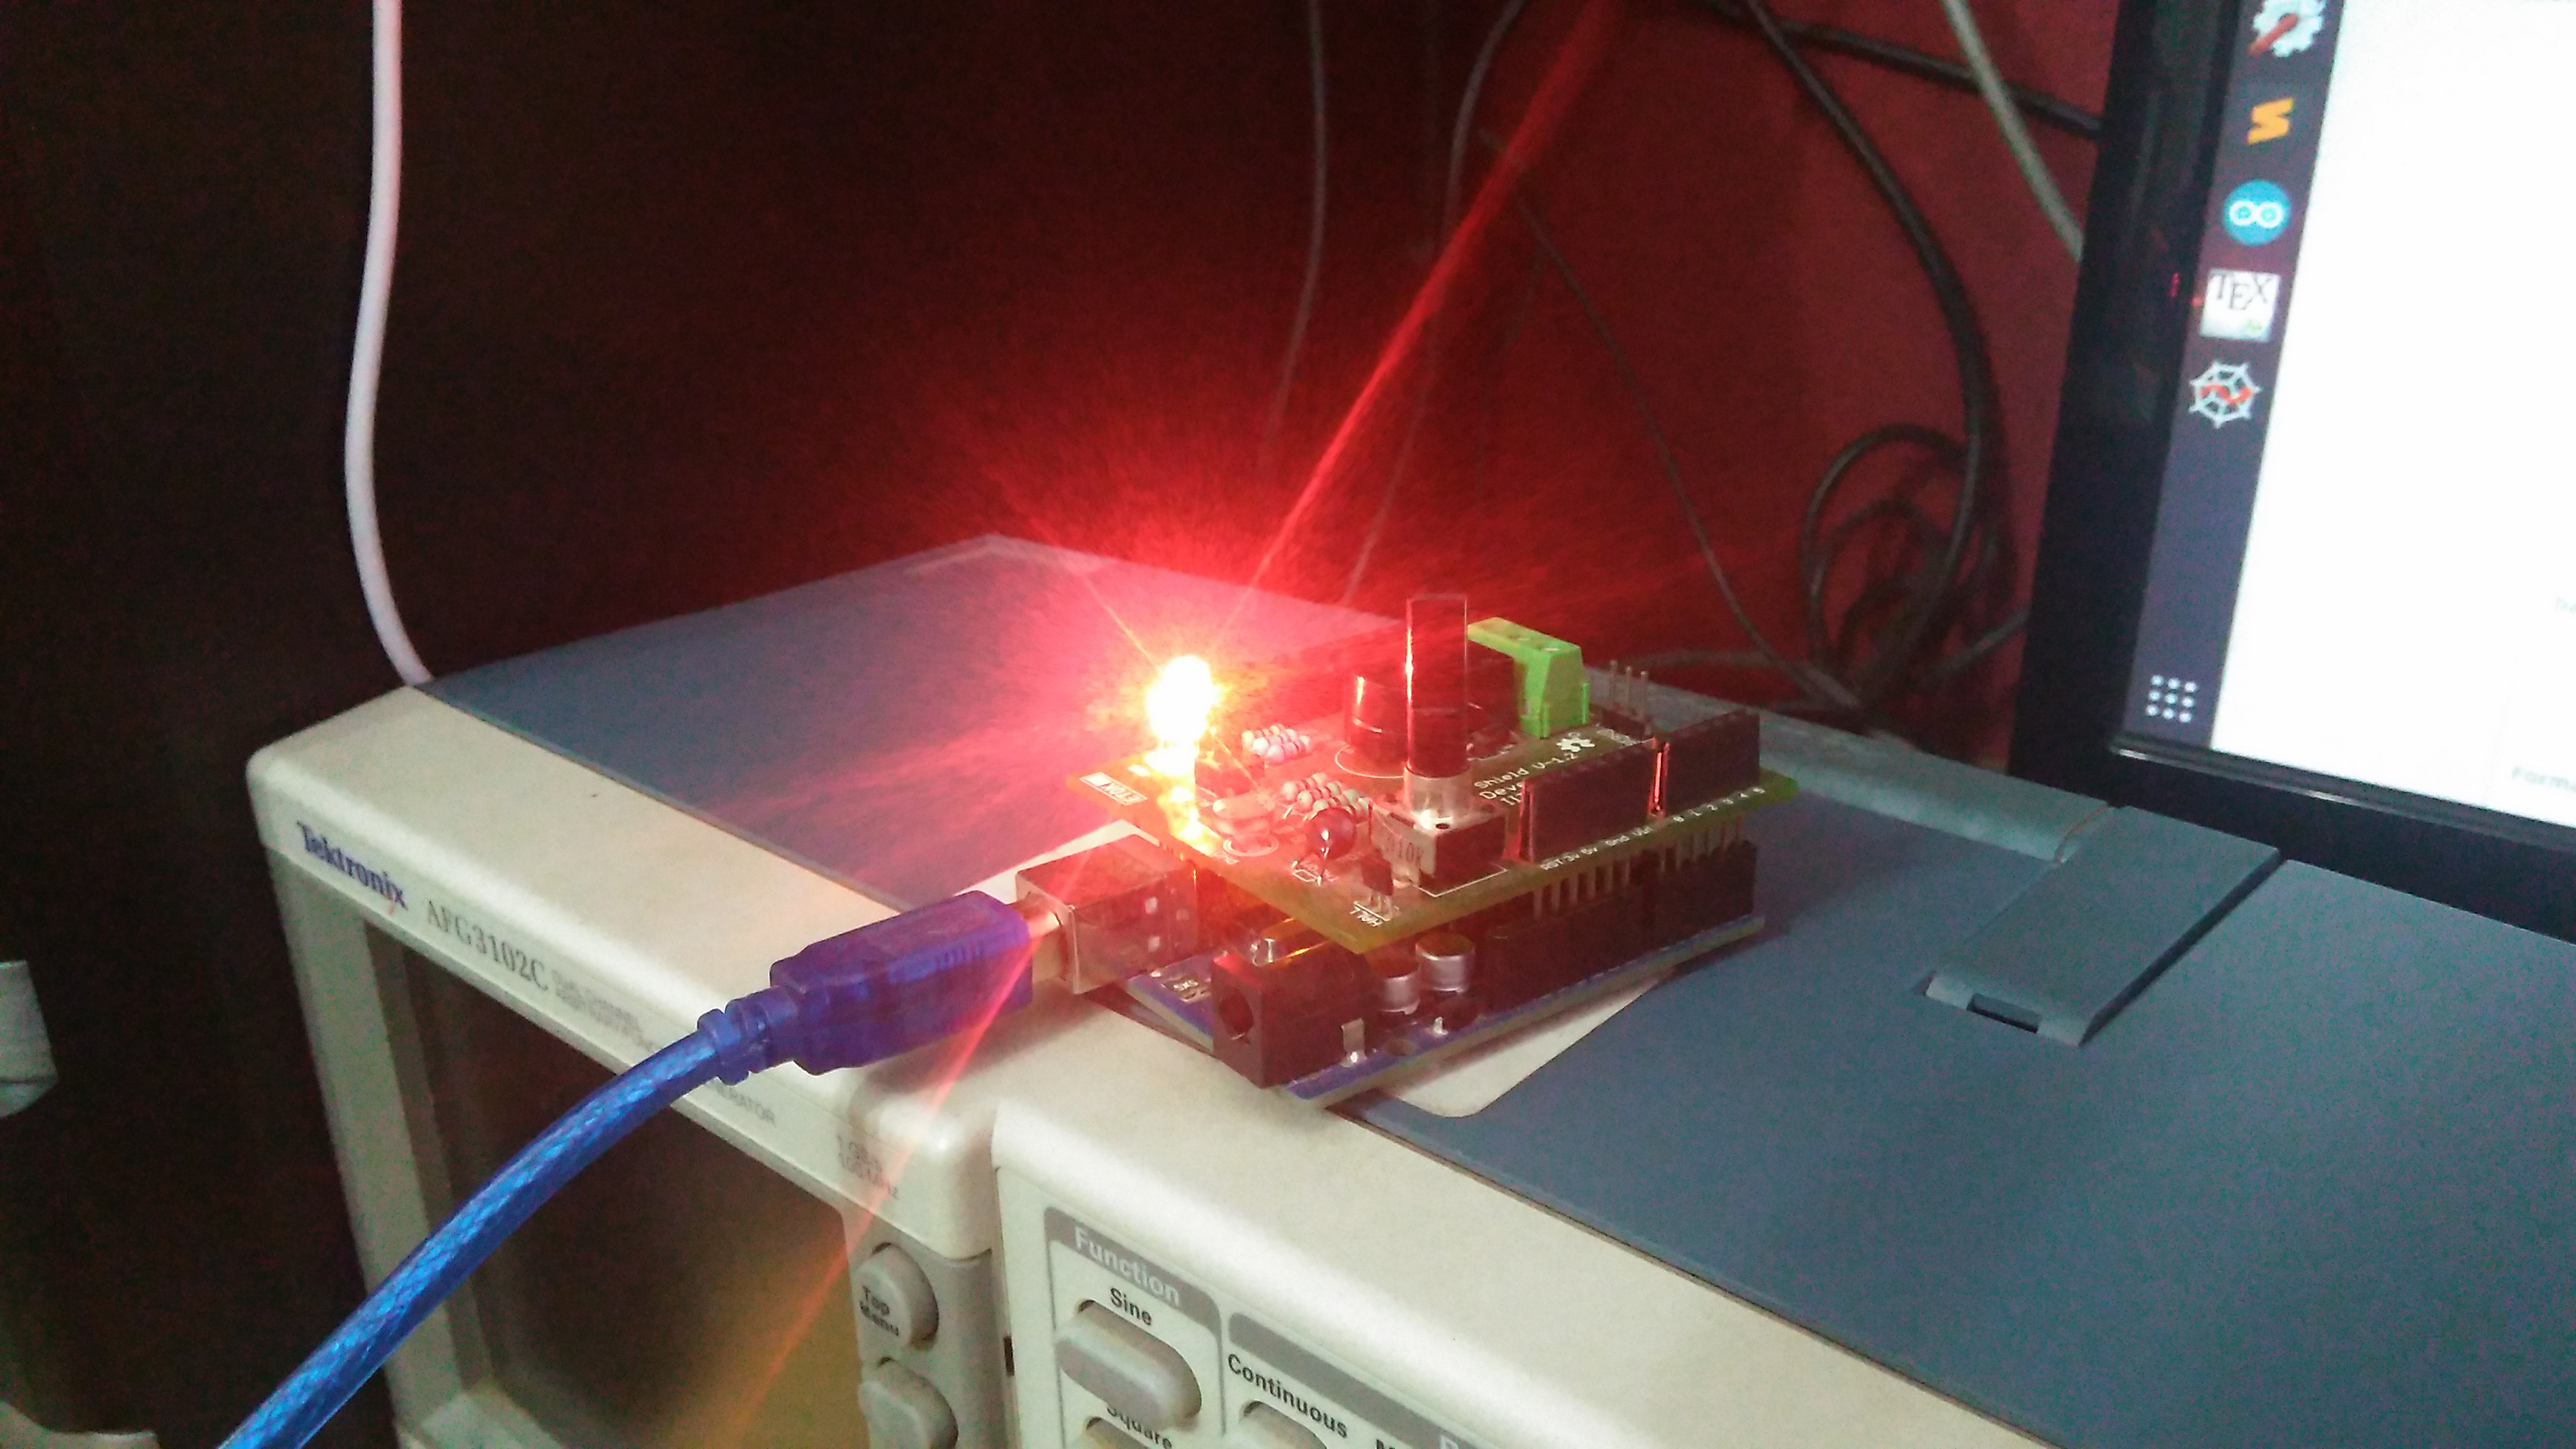
\includegraphics[scale=0.1]{Shield_With_Code.jpg}
\end{center}


\end{document}

